\documentclass{article} %basic LaTeX document type

%set capital Roman numeral section headings
%set capital Aramaic letters subsection headings
%set capital Arabic numbers subsubsection headings
\renewcommand\thesection{\Roman{section}.}
\renewcommand\thesubsection{\thesection\Alph{subsection}.}
\renewcommand\thesubsubsection{\thesubsection\arabic{subsubsection}.}

%set capital Roman numeral table numeration
\renewcommand*\thetable{\Roman{table}} 

%package needed for next lines
%makes section headings bold and upper case characters
%makes subsubsection headings in italics
\usepackage[explicit]{titlesec}
\titleformat{\section}{\bfseries}{\thesection}{1em}{\MakeUppercase{#1}}
\titleformat{\subsubsection}{\itshape}{\thesubsubsection}{1em}{#1}


%\linespread{2}       %option 1 for making text double-spaced
\usepackage{setspace} %option 2 for making text double-spaced
\doublespacing

%makes first paragraph of section indented (non-first are by default)
%set size of indentation (15pt is default)
\usepackage{indentfirst}
\setlength{\parindent}{25pt}

%set size of all margins
\usepackage[margin=1.3in]{geometry}
%can set margin sizes which are not the same in this way
%\usepackage[left=1in, top=1in, right=1in, bottom=1in]{geometry}

%package which returns number of last page (same as number of pages)
%package which counts the number of tables and/or figures
\usepackage{lastpage}
\usepackage[figure,table]{totalcount}

%enable `align' equation types
%enable `multirow' capability in tables
%enable figures
\usepackage{amsmath}
\usepackage{multirow}
\usepackage{graphicx}

%enables double spaced footnotes
\usepackage[]{footmisc}

%enables subfigures
%enables subfigure captions
%sets table caption formatting options to meet NSE requirements
%sets figure caption options to meet NSE requirements
\usepackage{caption}
\usepackage[labelformat=simple]{subcaption}
\captionsetup[table]{labelsep=newline,name=TABLE}
\captionsetup[figure]{name=Fig.,labelsep=period}

%sets labeling of footnotes
%double spacing of footnotes
\renewcommand{\thefootnote}{\alph{footnote}}
\renewcommand{\footnotelayout}{\doublespacing}

%enables proper labeling of subfigures
\renewcommand*\thesubfigure{(\alph{subfigure})}

%--------------
\usepackage{paralist}	
\usepackage{amssymb}
\usepackage{epsfig}
\usepackage[mathcal]{euscript}
\usepackage{setspace}
\usepackage{color}
\usepackage{array}
%\usepackage{subfigure}
\renewcommand{\ttdefault}{cmtt}
% The float package HAS to load before hyperref
\usepackage{float} % for psuedocode formatting
\usepackage{xspace}
\usepackage{mathrsfs}
\usepackage[pdftex]{hyperref}

%-------------
\DeclareMathOperator{\diag}{diag}
\DeclareMathOperator{\low}{lower}
\DeclareMathOperator{\upp}{upper}

\newcommand{\Sn}{\ensuremath{S_N}}
\newcommand{\Macro}{\ensuremath{\Sigma}}

\newcommand{\vOmega}{\ensuremath{\hat{\Omega}}}
\newcommand{\Ye}[2]{\ensuremath{Y^e_{#1}(\vOmega_#2)}}
\newcommand{\Yo}[2]{\ensuremath{Y^o_{#1}(\vOmega_#2)}}

\newcommand{\ve}[1]{\ensuremath{\mathbf{#1}}}

\newcommand{\sigg}[1]{\ensuremath{\sigma^{gg'}_{\text{s}\,#1}}}
\newcommand{\psig}{\ensuremath{\psi^g}}

\newcommand{\even}{\ensuremath{\phi^g}}
\newcommand{\odd}{\ensuremath{\vartheta^g}}

\newcommand{\evenp}{\ensuremath{\phi^{g'}}}
\newcommand{\oddp}{\ensuremath{\vartheta^{g'}}}

\newcommand{\apsi}[1]{\ensuremath{\psi^{\dagger\,#1}}}
\newcommand{\aeven}[1]{\ensuremath{\phi^{\dagger\,#1}}}
\newcommand{\aodd}[1]{\ensuremath{\vartheta^{\dagger\,#1}}}

\newcommand{\asigg}[1]{\ensuremath{\sigma^{g'g}_{\text{s}\,#1}}}

\newcommand{\aPsi}[1]{\ensuremath{\Psi^{\dagger\,#1}}}
\newcommand{\aPhi}[1]{\ensuremath{\Phi^{\dagger\,#1}}}

\newcommand{\epsi}{\ensuremath{\epsilon}}
\newcommand{\ephi}{\ensuremath{\varepsilon}}

\newcommand{\psie}{\ensuremath{\psi_{\epsi}}}
\newcommand{\phie}{\ensuremath{\phi_{\ephi}}}

\newcommand{\Psie}{\ensuremath{\Psi_{\epsi}}}
\newcommand{\Phie}{\ensuremath{\Phi_{\ephi}}}

\newcommand{\apsie}[1]{\ensuremath{\psi^{\dagger\,#1}_{\epsi}}}
\newcommand{\aphie}[1]{\ensuremath{\phi^{\dagger\,#1}_{\ephi}}}

\newcommand{\aPsie}[1]{\ensuremath{\Psi^{\dagger\,#1}_{\epsi}}}
\newcommand{\aPhie}[1]{\ensuremath{\Phi^{\dagger\,#1}_{\ephi}}}

\newcommand{\avg}[1]{\ensuremath{\langle#1\rangle}}

\newcommand{\osig}{\ensuremath{\overline{\sigma}}}
\newcommand{\osigs}{\ensuremath{\overline{\sigma_{\text{s}}}}}

\newcommand{\fwc}{\mbox{FW-CADIS}}

\begin{document}


%Define fields for \maketitle  (fields are \author, \date, \thanks, and \title)

\title{Assessment of the Lagrange Discrete Ordinates Equations for Monte Carlo Variance
Reduction Parameter Generation} %title of paper

\author{
\vspace{20mm}
%list of authors, with corresponding author marked by asterisk
\\Kelly L.\ Rowland,$^{\text{a}}$  Cory D.\ Ahrens,$^\text{b}$ Steven Hamilton,$^\text{c}$ 
\\and R.N.\ Slaybaugh$^{\text{a},\ast}$\\[4pt] 
%affiliations of authors
\textit{$^a$University of California, Berkeley, Nuclear Engineering Department}\\[-10pt]
\textit{4173 Etcheverry Hall, Berkeley, CA 94720, USA} \\[-5pt]
\textit{$^b$X Theoretical Design Division, Primary Physics Group}\\[-10pt]
\textit{Los Alamos National Laboratory, Los Alamos, NM 87545, USA}\\[-5pt]
\textit{$^c$Oak Ridge National Laboratory, Radiation Transport and Criticality Group} \\ [-10pt]
\textit{P.O. Box 2008, Oak Ridge, TN 37831-6170, USA} \\ [-2pt]
{$^\ast$slaybaugh@berkeley.edu}}       %address and email address for correspondence

%instead of returning the date, this repurposes the \maketitle command to print the number of pages, tables, and figures
\date{
\vspace{40mm}
Number of pages: \pageref{LastPage} \\  
Number of tables: \totaltables \\
Number of figures: \totalfigures \\}                                                                                           

\maketitle

\pagebreak

\begin{abstract}
{
abstract

Keywords: x; y; z
}
\end{abstract}

\pagebreak

%%---------------------------------------------------------------------------%%

\section{Introduction}
\label{sec:intro}

\begin{itemize}
\item{3D neutron transport is on the rise with HPC}
\item{Discrete ordinates and Monte Carlo are common solution approaches}
\item{Hybrid methods aim to leverage the strengths of both}
\end{itemize}

%%---------------------------------------------------------------------------%%
%%---------------------------------------------------------------------------%%
%%---------------------------------------------------------------------------%%
\section{Background}
\label{sec:background}
%%---------------------------------------------------------------------------%%
%%---------------------------------------------------------------------------%%
\subsection{Denovo}

\begin{itemize}
\item{Denovo is the transport solver in the Exnihilo code suite developed at
ORNL}
\item{2D and 3D neutral particle transport}
\item{Scalable}
\end{itemize}

%%---------------------------------------------------------------------------%%
%%---------------------------------------------------------------------------%%
\subsection{LDO Equations}

\begin{itemize}
\item{Developed by Ahrens}
\item{Inherently 3D}
\end{itemize}

%%---------------------------------------------------------------------------%%
%%---------------------------------------------------------------------------%%
%%---------------------------------------------------------------------------%%
\section{Past Work}
\label{sec:pastwork}
% replace this with a 'methodology' sort of section?

%%---------------------------------------------------------------------------%%
\section{Results}
\label{sec:results}

\begin{itemize}
\item{Compared LDO equations' associated MC VR parameters with those from standard quadrature 
      sets}
\item{Relatively coarse multigroup energy library}
\end{itemize}

%%---------------------------------------------------------------------------%%
%%---------------------------------------------------------------------------%%
\subsection{Steel Plate Embedded in Water}

The first test case we describe is an idealized geometry of a steel plate embedded in
water; it is modeled after the scenario presented in Reference 
\cite{wilsonslaybaugh}. 
A diagram of the problem geometry is shown in Figure \ref{steelxz} and a list
of material properties used in the problem is given in Table \ref{steel-mat}.
In Figure \ref{steelxz}, the orange region contains the source material, the black
region is composed of steel, the blue regions indicate water, and the white region is
composed of air.

\begin{figure}[!htb]
\centering
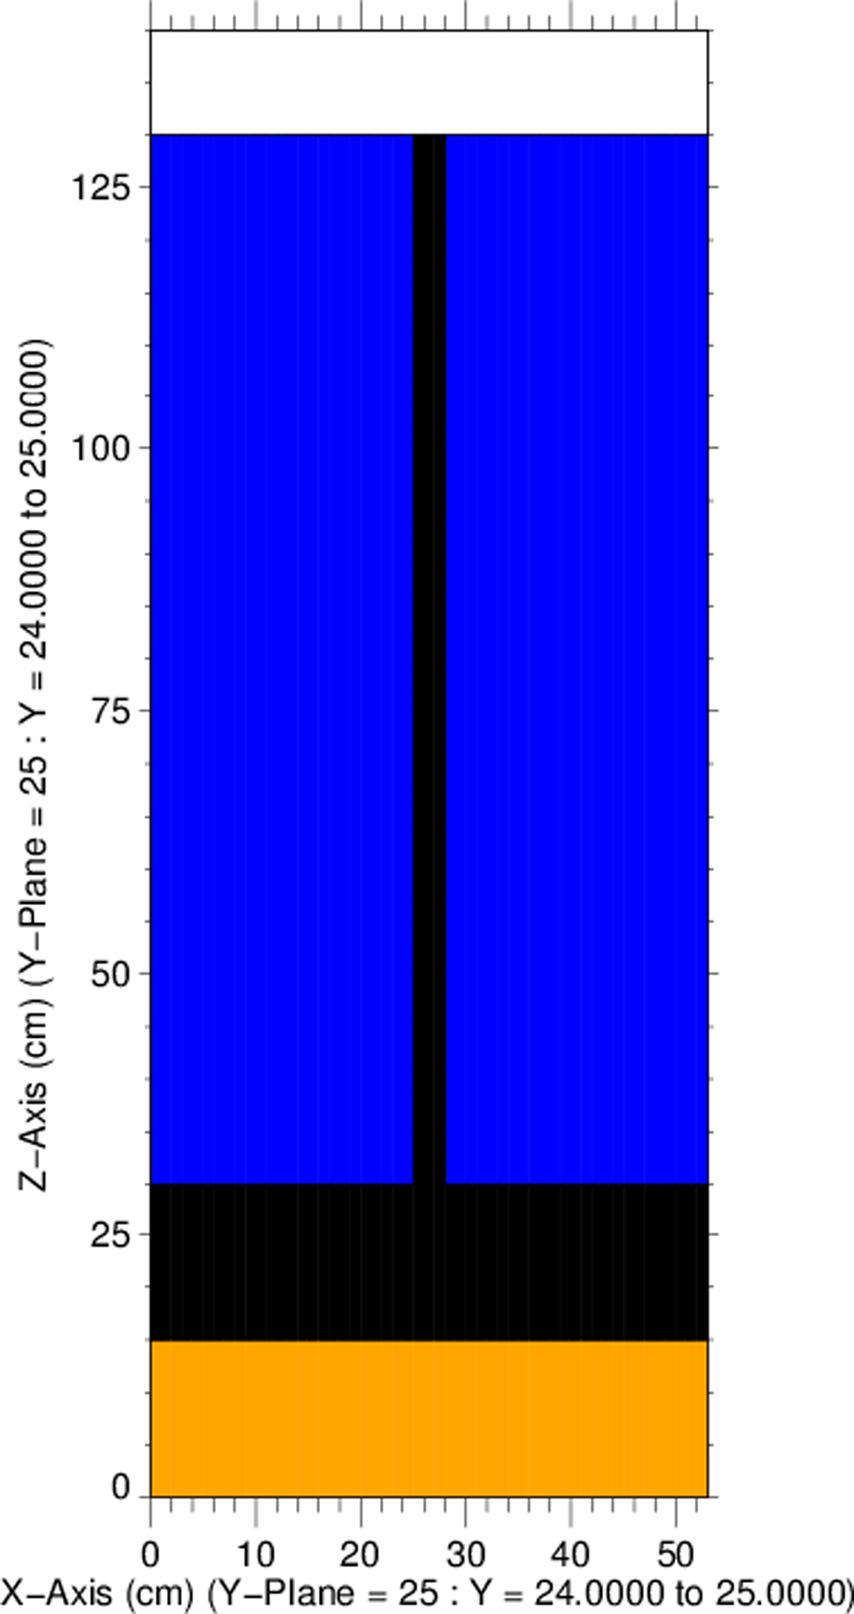
\includegraphics[width=0.4\textwidth]{img/steel-xz.png}
\caption{Steel plate in water geometry ($x-z$ slice through $y = 25$ cm) 
         \cite{wilsonslaybaugh}.}
\label{steelxz}
\end{figure}

The problem measurements are $53\times50\times140$ cm. The scenario is uniform in the 
$y$-direction and materials vary mainly in the $z$-direction. The source region 
extends from 0 to 15 cm, the steel shield extends between 15 and 30 cm, the water and 
steel plate extend from 30 to 130 cm, and the air extends from 130 to 140 cm. The 
steel plate is 3 cm wide and is centered at $x = 26.5$ cm. Vacuum boundary conditions 
were used at the problem boundaries.

A non-uniform Cartesian mesh was used for the spatial discretization in the 
deterministic calculations. In the $x$-direction, voxel width is 5 cm between $x = 0$
cm and $x = 25$ cm, 0.5 cm between $x = 25$ cm and $x = 28$ cm, and 5 cm between 
$x = 28$ cm and $x = 53$ cm. A uniform spacing of voxel width 1 cm was used in the 
$y$-direction. In the $z$-direction, the spatial cell width is 3 cm between $z = 0$ cm and
$z = 30$ cm and 2 cm between $z = 30$ cm and $z = 140$ cm.

\begin{table}[!htb]
\centering
\caption{Materials and compositions in the steel plate in water scenario.}
\label{steel-mat}
\begin{tabular}{l|cc}
Material & \multicolumn{2}{c}{Isotopes (Atomic \%)} \\ \hline
\multirow{5}{*}{Source}   & U-235   & (0.000247) \\
                          & U-238   & (0.009287) \\
                          & Zr-nat. & (0.004009) \\
                          & H-1     & (0.037394) \\
                          & O-16    & (0.034927) \\ \hline
\multirow{4}{*}{Air}      & N-14    & (0.784431) \\
                          & O-16    & (0.210748) \\
                          & Ar-nat. & (0.004671) \\
                          & C-nat.  & (0.000150) \\ \hline
\multirow{2}{*}{Carbon Steel} & C-nat.  & (0.022831) \\
                              & Fe-nat. & (0.977169) \\ \hline
\multirow{2}{*}{Water}        & H-1     & (2)        \\
                              & O-16    & (1)        \\
\end{tabular}
\end{table}

The composition of the neutron source block is a homogenization of water, zirconium,
and uranium and was calculated based on the geometry and composition of the Rowlands
UO$_2$ pin cell benchmark specification \cite{pincell}. The source is a U-235 fission 
spectrum that is uniformly distributed throughout the homogenized material. The
compositions of air, carbon steel, and water were taken from the Compendium of 
Material Composition Data for Radiation Transport Modeling \cite{pnnl}.

%%---------------------------------------------------------------------------%%
%%---------------------------------------------------------------------------%%
\subsection{Dog-Legged Void Neutron}

The next problem modeled is the dog-legged void neutron (DLVN) experimental benchmark,
which was designed to measure neutron streaming in iron with air voids. The model used
in the following calculations was constructed from References 
\cite{sw-dlvn,j-dlvn,dlvn1991}. The two materials used in the problem are elemental 
iron and polyethylene. The polyethylene composition used was C$_2$H$_4$. This is 
listed as ``polyethylene, non-borated'' and is material 248 in Reference \cite{pnnl}. 

\begin{figure}[!htb]
\centering
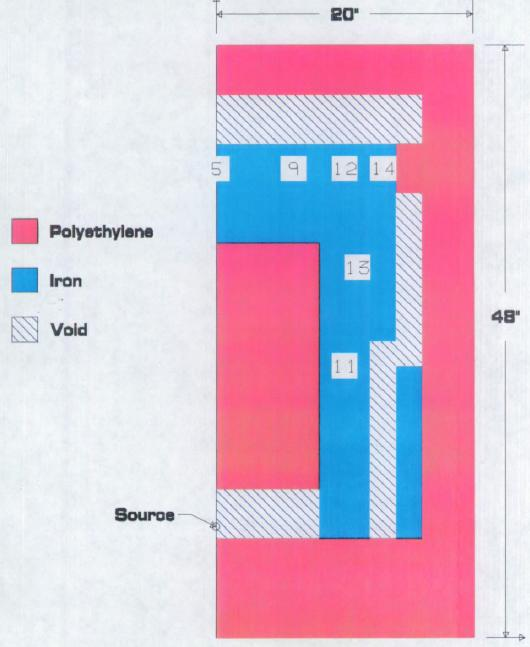
\includegraphics[width=0.5\textwidth]{img/dlvn.png}
\caption{Centerline cutaway of DLVN setup \cite{sw-dlvn}.}
\label{dlvn}
\end{figure}

The problem measurements are $40\times54\times48$ inches. A uniform spatial mesh was 
imposed over the entire problem, with voxels measuring 1 inch per side. The neutron
source in this problem is a Cf-252 point source located at the center of the $x-$ and
$y-$directions and at $z = 9$ inches.
This point source was approximated as a small volumetric source in the tests in this 
work.

The experimental configuration is symmetric about the $y-z$ plane at $x = 0$ and so is
usually simulated with a reflecting boundary at $x = 0$ and vacuum boundaries on all
other sides of the configuration. For the tests in this work, the use of reflecting
boundary conditions was not available, so the model used 
was constructed to represent the entire experimental geometry configuration. Vacuum
boundary conditions were applied to the outside of the entire problem.

%---------------------------------------------------------------------------%%
\section{Conclusions}
\label{sec:conclusions}

\pagebreak
\section*{Acknowledgments}

This material is based upon work supported under an Integrated
University Program Graduate Fellowship as well as supported by the Department 
of Energy under Award Number(s) DE-NE0008661. This report was prepared as an
account of work sponsored by an agency of the United States Government.
Neither the United States Government nor any agency thereof, nor any of their
employees, makes any warranty, express or limited, or assumes any legal
liability or responsibility for the accuracy, completeness, or usefulness of
any information, apparatus, product, or process disclosed, or represents that
its use would not infringe privately owned rights. Reference herein to any 
specific commercial product, process, or service by trade name, trademark, 
manufacturer, or otherwise does not necessarily constitute or imply its 
endorsement, recommendation, or favoring by the United States Government or
any agency thereof. The views and opinions of authors expressed herein do not 
necessarily state or reflect those of the United States Government or any 
agency thereof. This research used the Savio computational cluster resource provided by the 
Berkeley Research Computing program at the University of California, Berkeley 
(supported by the UC Berkeley Chancellor, Vice Chancellor for Research, and Chief 
Information Officer).

\pagebreak

\bibliographystyle{nse}
\bibliography{ldo-mc-vr}

\end{document}

